\chapter{Diagnostika a detekce anomálií} \label{chap:diagnostics}
Systém diagnostiky chyb a detekce anomálií je v projektu chytré domácnosti rozdělen do tří úrovní - detekce chyb na úrovni mikročipu ESP8266, detekce anomálií na základě klasifikace z natrénovaného modelu a diagnostika stavu čidel na serveru. Všechny části diagnostického systému jsou popsány v této kapitole. 

\subsection*{Význam diagnostického systému}
Smyslem využití systému detekce anomálií je automatická diagnostika senzorů na základě příchozích zpráv. Výstupem tohoto systému je informace o stavu klientů. Stavy jednotlivých senzorů se propisují do webové vizualizace (více v \cref{chap:web_page}) a díky ikonám vedle měřených veličin dostává uživatel okamžitý a kompletní přehled o stavu senzorů v chytré domácnosti. Zároveň má jistotu, že data zobrazovaná na webové stránce jsou aktuální, protože diagnostický systém ví, že data ze senzorů mají chodit pravidelně s pevnou periodou a když nové hodnoty nepřijdou, upozorní na to změnou ikony. Uživatel se tedy dozví, že senzor nepracuje stoprocentně a zobrazená data nemusejí být relevantní.

- Proč řešit diagnostiku čidel v rámci chytré domácnosti, ...\\
- Úvod do detekce anomálií, základní principy, smysl využití, ... - možná přidat ještě nějakou větu..

\subsection*{Výstup systému detekce anomálií}
Výstupem systému diagnostiky chyb a detekce anomálií jsou tři stavy přiřazené jednotlivým senzorům. Senzor se může nacházet v jednom z těchto tří stavů. 

\begin{itemize}
  \item \textit{Sensor OK} je stav senzoru, kdy všechno funguje bezproblémově; Senzor odesílá data tak, jak se očekává - periodicky každou minutu a naměřená hodnota odpovídá natrénovanému modelu (více v \cref{sec:detection_classification}); Ikona pro tento stav je zelená.
  \item Stav \textit{Value ERROR} nastává, pokud senzor odesílá data periodicky - tak, jak se očekává, ale naměřená hodnota je mimo předpovězený rozsah - neodpovídá natrénovaném modelu; Tento stav je tedy mezi stavy "Sensor OK" - kdy je vše v pořádku a "Sensor ERROR" - kdy senzor nefunguje vůbec; Ikona pro tento stav má žlutou barvu.
  \item \textit{Sensor ERROR} je status čidla, který nastává v momentě, kdy čidlo neposílá žádná data; Tento stav je způsobený pravděpodobně výpadkem čidla nebo nedostupností internetu; Tento status senzoru popisuje červená ikona.
\end{itemize}

Na \cref{fig:markovov_diagram} je zobrazeno schéma Markovova řetězce, který popisuje přechody mezi jednotlivými stavy senzorů. Z tohoto řetězce je patrné, že každý stav může přejít do libovolného jiného stavu nebo zůstat v aktuálním stavu. To znamená, že pokud se čidlo nachází v jednom momentě například ve stavu "sensor OK", v následujícím momentě se může nacházet opět ve stavu "OK"\ nebo v libovolném jiném stavu - "value ERROR"\ nebo "sensor ERROR".

\begin{figure}[H]
  \centering
  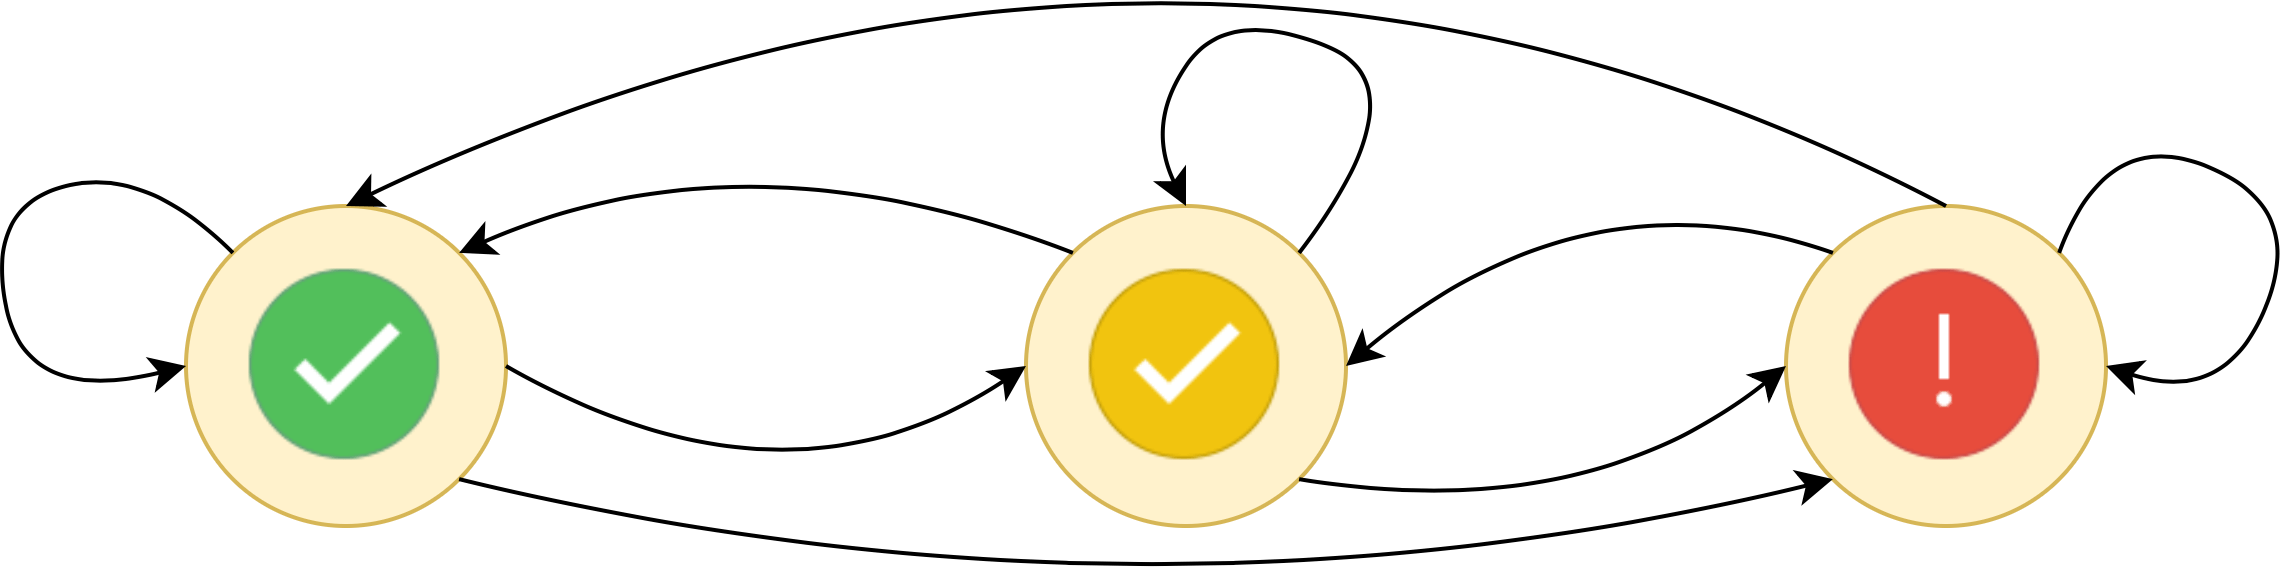
\includegraphics[width=0.6 \textwidth]{markovov_diagram.png}
  \caption{Markovův řetězec popisující přechody mezi jednotlivými stavy senzorů}
  \label{fig:markovov_diagram}
\end{figure}  

\section{Detekce chyb na úrovni ESP8266} \label{sec:error_detection_esp}
První a nejnižší úroveň diagnostiky jednotlivých senzorů je detekce chyb na úrovni samotného mikročipu. Mikročip ESP8266 při každém načítání dat z čidla zkouší, jestli z daného čidla lze načíst data a pozná, když je čidlo nefunkční. Čidlo se považuje za nefunkční, pokud při vyžádání naměřených dat nevrací žádné hodnoty. Tento stav čidla může být způsobený špatným zapojením, vypojením čidla nebo rozbitým čidlem. Implementace detekce chyb na úrovni mikročipu spočívá v obsluze výjimek v kódu. Část kódu, která řeší komunikaci s čidlem je obalena v \textit{try-except} bloku - mikročip se snaží načíst data z čidla a v případě, že to nelze, spadne kód do části \textit{except}, kde se obslouží výjimka tím, že se do proměnné, kam se ukládá naměřená hodnota, přiřadí číslo -1. Cyklus v kódu pokračuje dále k vytváření struktury zprávy, kde se testuje, zda se hodnota v proměnné nerovná -1. Pokud ano, ve zprávě se změní hodnota atributu "status"\ na "error"\ a senzor odešle zprávu (více o programování mikročipu v \cref{subsec:periodical_based_msg}). Senzor tedy odesílá zprávy na broker vždy - s funkčním i nefunkčním čidlem a status zprávy v detekci chyb na této úrovni nabývá pouze dvou hodnot - "ok"\ a "error". \par
Implementací detekce chyb na úrovni mikročipu byla zajištěna robustnost senzorů. Jednotlivé senzory jsou odolné vůči výpadkům čidel - kód na mikročipu nespadne kvůli nefunkčnímu čidlu, jen se změní status zprávy. Díky tomu je také zajištěn nonstop provoz - čidla lze k ESP8266 připojovat a odpojovat (například čidlo teploty nebo magnetické kontakty, které jsou připojeny přes konektor) v reálném čase bez nutnosti restartu mikročipu. Pokud čidlo v jakémkoliv časovém okamžiku odpojím a po chvíli zase připojím, mikročip si s tím poradí. Změní se status zprávy a celý systém funguje dál. \par
Výhoda implementace detekce chyb na úrovni mikročipu se během testování ukázala několikrát. Například když jsem potřeboval vyměnit nefunkční čidlo vlhkosti DHT11, které je připojené přes dutinkovou lištu (více v \cref{subsec:dht11}), jen jsem vyměnil kus za kus a senzor okamžitě začal načítat data z čidla a posílat naměřené hodnoty.

\section{Detekce anomálií na základě klasifikace} \label{sec:detection_classification}

Ve skriptu engine.py jsou příchozí data z brokeru klasifikována a následně odesílána na webovou stránku. Klasifikace -1 nebo 1 podle... Webová stránka dále pracuje s klasifikací - zobrazení ikon u jednotlivých veličin (zelená, žlutá, červená)

- pozn.: vlhkost v místnosti se mění s ročním obdobím - v zimně kolem 40-50 procent, v létě kolem 20-30 procent..
- Implementace funkcí scikit-learn pro natrénovaní modelů \\
- Nastavení modelu a natrénování modelů pro jednotlivé veličiny \\
- Porovnání schémat natrénovaných modelů \\
- Implementace do projektu - klasifikace jednotlivých příchozích zpráv (přidání atributu "classification" do každé zprávy)
- Implementace detekce anomálií přijatých zpráv na základě rozhodnutí klasifikace - klasifikace 1 nebo -1 (1 v případě, že přijatá zpráva svou hodnotou "odpovídá" natrénovanému modelu, -1 v případě, že se vychyluje od natrénovaného modelu) \\
- Přenos této informace o klasifikaci do webového rozhraní \\

\section{Diagnostika stavu čidel na serveru} \label{sec:error_detection_server}
Diagnostika stavu čidel na úrovni serveru spočívá v implementaci funkce \textit{sensor\_check}, která běží ve skriptu \textit{engine.py} v backendové části serveru (popsáno v \cref{sec:webserver}). Systém diagnostiky na této úrovni spojuje předešlé dvě úrovně detekce chyb. Pracuje současně s informací o stavu na úrovni mikročipu (popsáno v \cref{sec:error_detection_esp}) a s informací o klasifikaci (popsáno v \cref{sec:detection_classification}). Funkce \textit{sensor\_check} kontroluje pravidelnost odesílání dat ze senzoru na broker. Pokud čidlo z neznámého důvodu neodešle zprávu nebo pokud se zpráva nepřenese k brokeru, informace o anomálii se přenese do webového rozhraní. Na \cref{fig:status_error} je ukázka příkladu zobrazení chyby senzoru ve webové vizualizaci. V případě chyby senzoru se změní ikona statusu a hodnota měřené veličiny je automaticky 0. Více o webové vizualizaci v \cref{sec:overview}.

\begin{figure}[H]
  \centering
  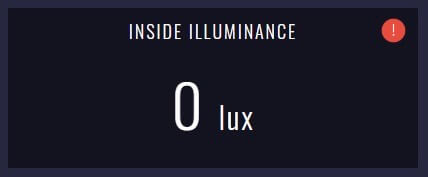
\includegraphics[width=0.4 \textwidth]{status_error.jpeg}
  \caption{Zobrazení ve webové vizualizaci v případě chyby senzoru}
  \label{fig:status_error}
\end{figure} 

Funkce \textit{sensor\_check} je implementována ve třídě MQTT Client a v novém vlákně běží paralelně vedle ostatních metod. Tato funkce čte všechny příchozí zprávy a porovnává čas poslední přijaté zprávy od daného čidla s aktuálním časem. Jestliže je rozdíl těchto dvou proměnných (čas poslední přijaté zprávy mínus aktuální čas) větší než zvolená mez, funkce detekuje chybu, do terminálu vypíše ID senzoru, ve kterém se vyskytuje chyba a status tohoto senzoru změní na "sensor ERROR". V tomto projektu byla zvolena 60 vteřinová mez, což znamená, že stačí, aby senzor jednou neodeslal zprávu a hned je považován za vadný. Toto kritérium je relativně přísné, v běžném provozu by stačilo mez volit například 180 vteřinovou, tudíž by se ve webovém rozhraní zobrazoval senzor jako aktivní i když by dvakrát neodeslal zprávu. Tři minuty staré data lze považovat za stále aktuální a stav senzorů by byl více konzistentní - občas se stane (ne příliš často, například jednou za 2 dny provozu), že senzor z nějakého důvodu nestihne odeslat zprávu v dané minutě a webová vizualizace ho ihned vyhodnotí jako nefunkční, přitom senzor v dalších minutách opět zprávy odesílá. Status senzoru se zbytečně rychle změnil a uživatel by mohl být zmatený. 

\subsection*{Hierarchie statusů}
Ve webovém rozhraní se mění ikony statusu podle tří stavů, které jsou popsány na výše definovaných úrovní. Statusy se mohou navzájem přepisovat podle hierarchie důležitosti, která je následující. 

\begin{lstlisting}[language=json]
	   Sensor ERROR > Value ERROR > Sensor OK
\end{lstlisting}

To znamená, že pokud senzor například odešle zprávu se statusem "sensor OK", ale hodnota měřené veličiny je klasifikována jako -1, na webu se zobrazí status odpovídající klasifikaci -1 - "value ERROR", protože status "value ERROR"\ má větší váhu, než status "sensor OK". \par
Pokud senzor odešle zprávu se statusem "sensor ERROR", tato zpráva není dále klasifikována a na webové stránce se zobrazí ikona "sensor ERROR". Váha tohoto statusu je nejvyšší. \par
Pokud senzor odešle zprávu se statusem "sensor OK"\ a klasifikátor přiřadí hodnotu 1, ikona statusu na webu zůstává "sensor OK". \par
Když senzor odešle zprávu se statusem "sensor OK", ale pak několik minut po sobě přestane odesílat zprávy, na webu se status změní na "sensor ERROR". \par
Diagnostika a změny ikon zpráv jsou zkrátka řešeny tak, aby to bylo pro uživatele přirozené a na první pohled pochopitelné. Zelená ikona znamená, že je všechno v pořádku. Žlutá ikona uživateli říká, že je všechno víceméně v pořádku, ale něco není úplně stoprocentně správně. Červená ikona uživatele varuje a říká, že je senzor nefunkční. Diagnostický systém kombinuje vstupy ze systému kontroly stavu čidel s kontrolou věrohodnosti posílaných zpráv a kontrolou pravidelností odesílaných zpráv. Kombinací těchto tří subsystémů generuje výstupní ikony na webové stránce, které informují uživatele.